%% Sample chapter file, for use in a thesis.
%% Don't forget to put the \chapter{...} header onto each file.

\chapter{Introduction}{

\section{The Internet of Things Era}{

The past decades were the decades when the World-Wide-Web penetrated our life. As the time passes and technology advances, humans find more clever ways to integrate Internet technology to improve our lives, become more efficient and tackle problems that previously seemed impossible. Robotics, virtual reality, the Internet of Things, the cloud and artificial intelligence move from the pages of science-fiction books to the reality. Utilizing these novel technologies is expected to make a new industrial revolution and reshape the industry entirely. For that reason, governments around the globe form their strategic plan around arising technology. The German government has already published their high-tech policy that aims to reform their industry, called \textit{Industry 4.0} \cite{lasi2014industry}. Meanwhile, the Chinese government is pushing an initiative to comprehensively upgrade their industry, \textit{Made in China 2025} \cite{kennedy2015made}, which is based on the applications of new technology to reform the manufacturing and supply chain industries.

A core part of this technological revolution is the Internet of Things (IoT). IoT can be defined as a set of connected devices that are capable of communicating with the rest of world in the form of sending and receiving data via the Internet \cite{said2013towards}. IoT shines in industrial applications, as it provides a mean of communication between machines and computers. This communication could be used to collect data during operation and to proactively take action based on the data. However, IoT applications are not limited to the industrial environment. Smart-homes, fitness trackers and autonomous cars are domains in which IoT has its rightful place. With all those applications of IoT devices we expect a dramatic increase in its adoption rate. In particular, ARM predicts the number of use cases of IoT will increase and exponentially and that 1 trillion IoT devices will be deployed by 2020 \cite{Sparks2017TheDevices}. The exponential increase int the number of IoT devices creates the need for efficiency in every aspect of an IoT device. The devices need to collect data, process data, communicate with the Internet and update their firmware efficiently.
}

\section{Firmware Distribution}{

Updates are a crucial part in the lifetime of any software. Software updates are the only reliable way to make a software stand against the test of time. Software updates add features, improve the efficiency and remove bugs from the software. Besides performance, software updates also fix security vulnerabilities, improve the security of the system and address known and potential attacks against the software. Consequently, it would be wishful thinking to imagine a software that does not need any update in its lifetime. However, especially in the case of IoT devices and firmware updates, updating is are one of the most vulnerable phases in the lifetime of the device \cite{Shamir2017SummaryCryptography}. The reason for that, is the high computational cost entailed in applying cryptographic primitives. As a result, many manufacturers tend to either not use them at all or use insecure implementations.

Firmware distribution is a specific type of content distribution that aims at delivering a single firmware file with a size of ~5-15 MBytes from a firmware developer to an end device. Traditionally the architecture of firmware updates for IoT devices is the one illustrated in Figure \ref{fig:FirmUpd}. The IoT gateway (i.e. a personal computer or a smartphone) will download the firmware from the manufacturer server. Then the gateway will verify the origin of the firmware based on a specified code signing protocol and push the firmware to the end-device using a Wireless Local Area Network (WLAN) protocol such as Bluetooth \cite{fitbit}.

\begin{figure}[htb!]
\centering
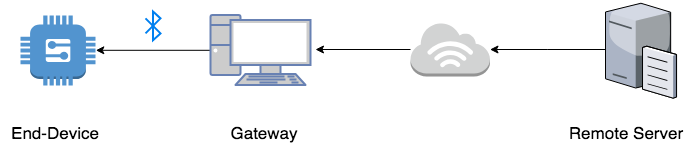
\includegraphics[width=0.95\textwidth]{./pics/Firmware_updates.png}
\caption{Traditional IoT architecture for distributing firmware updates}
\label{fig:FirmUpd}
\end{figure}

Firmware updating, is such a sensitive process that it spawned a new attack surface against embedded devices called firmware-modification attacks \cite{7804660}. Firmware modification attacks can have devastating effects on the device. Modified firmware can transform the device into a spyware and steal sensitive information from the user. They can disable the device bootloader, thus making it extremely hard to update the firmware of the device and remove the malicious firmware. In general, once a malicious firmware is injected, the device becomes the hostage of the attacker. Interested readers can refer to the paper of Classen et. al. that illustrates different attacks that rely on the firmware-modification attack \cite{Classen2018AnatomyFirmware}.
}

\section{Problem Definition} \label{sec:PD}{

In this project we aim to develop a decentralized firmware update network that would enable open-source development of IoT firmware. Open-source development of firmware benefits are twofold. Firstly, it enables patching vulnerable firmware even if the device manufacturer goes bankrupt. Secondly, open-source development enables transparency and code review. The user can review the code to know exactly what data are gathered from her and how they are being used. This transparency is crucial given the nature of IoT applications in home automation and wearable devices.

For our decentralized firmware update network we set the following requirements:
\begin{itemize}
    \item \textbf{No single point of failure}: The users should be able to retrieve a new firmware even in the case that a single node fails. Making the system resistant to single point of failures will also implicitly allow open-source development of firmware. Device manufacturers may have an advantage over others, however this advantage should not prohibit developers from developing new firmware for a device. 
    \item \textbf{Equivalent security with code signing}: The system should not make any security discounts over the current status quo, which is code signing.
    \item \textbf{Transparency}: Firmware updates should be eponymous, immutable and persistent. Any user should be able to retrieve and browse through the firmware releases for a given device.
    \item \textbf{Scalability}: The firmware release should be distributed and evenly balanced. Nodes participating in the network should contribute by uploading firmware they have to other peers and be able to download firmware they want from peers.
\end{itemize}

}

\section{Our Contribution}{

The goal of this project is to design a decentralized firmware update framework for IoT devices. To that end, we contributed in the following ways:

\begin{enumerate}
    \item We developed a smart-contract that models trust in decentralized environments. The implementation was based on the idea of Web-of-Trust. To our knowledge there is no publicly available implementation of Web-of-Trust in an Ethereum smart-contract.
    \item We developed a smart-contract that performs the business logic of a firmware repository. The firmware repository is feeless for the users and the fees required by the developers are minimal.
    \item We designed and developed the Código network clients that meet the requirements set in Section \ref{sec:PD}. Código network interacts with the Ethereum and IPFS networks in a user-friendly way. We measured the costs entailed in using the Código network.
    \item We designed a simulation tool to measure the performance of IPFS and used this simulation tool to compare the performance of IPFS against the Client-Server model and BitTorrent.
    \item The  features we added to the IPFS simulation framework and the performance results received attention from the IPFS community \footnote{\url{https://github.com/ipfs/go-ipfs/issues/5226}} and spawned a fruitful discussion on the current implementation. Our findings point to the main performance issues of IPFS. Additionally, we made the first comparison between IPFS and BitTorrent. The developed code is now under code-review in order to be included in the IPFS testing framework.
\end{enumerate}

}

\section{Project Outline}{

The rest of this project is organized as follows: Chapter \ref{chap:bc} aims to provide the reader with sufficient background information on Blockchain technology and Ethereum decentralized applications, in order to understand the evaluation of Código network smart-contracts.  Chapter \ref{chap:cn} presents and compares the most common approaches used for file distribution. Chapter \ref{chap:CNDesign} documents our design of Código network. In this part, we focus on modeling trust and implementing the smart-contracts and the UI clients developed. Additionally, the performance of the developed Ethereum smart-contracts, measured in terms of transaction costs, is presented. For completeness we evaluate closely related work. In Chapter \ref{chap:CNeval} a comparison between different file distribution frameworks is presented. Additionally, the experiment setting and the simulation frameworks developed and used to perform the comparisons are presented. In chapter \ref{chap:conc}, an overall analysis of completion of the project is presented. The assessment is based on the requirements set in Section \ref{sec:PD} and some ethical consideration that arose during the project are presented. Finally, the project is concluded with proposals for further research.

}

}
